\apendice{Especificación de Requisitos}

\section{Introducción}
En este apéndice se recogerán los diferentes objetivos del proyecto con sus correspondientes requisitos funcionales y no funcionales que marcan el desarrollo de este proyecto.

\section{Objetivos generales}

Este proyecto tiene como objetivo el desarrollo de un modelo que nos permita predecir la presencia de medusas en las costas de Chile en función de las condiciones marítimas. El modelo resultante se utilizará en un aplicación web con la que poder consultar la predicción de la fecha requerida ayudando a su visualización mediante representaciones gráficas.

\section{Catálogo de requisitos}

	\subsection{Requisitos funcionales}

\begin{description}
	\item[RF-1 Obtención de los datos:] Se debe ser capaz de descargar los datos necesarios de manera automática a través de un servidor FTP.
	\item[RF-2 Filtrado de los datos:] Los datos descargados han de ser tratados, descartando las zonas geográficas distintas al lugar de estudio así como las variables ambientales que no sean de utilidad.
	\item[RF-3 Cruce de datos:] Los datos filtrados se han de cruzar con los de avistamientos, obteniendo una estructura de los avistamientos con su respectiva fecha, localización y variables oceánicas.	
	\item[RF-4 Consultar modelo:] La aplicación debe ser capaz de realizar una consulta al modelo predictivo a partir de los datos introducidos por el usuario.
	\item[RF-5 Mostrar mapa:] La aplicación debe ser capaz de mostrar un mapa con el que poder interactuar.
	\item[RF-6 Introduccion de datos para su visualización:] El usuario debe poder seleccionar una serie de datos con los que realizar las consultas.
	\subitem RF-6.1 Elección de fechas: Se debe poder seleccionar una fecha de la que obtener información.
	\subitem RF-6.2 Elección de playa: Se debe poder elegir una playa de la que obtener información.
	\subitem RF-6.3 Visualización de resultados: El usuario debe ser capaz de visualizar los resultados de una playa en la fecha especificada.	
	\item[RF-7 Exportación de resultados:] Se deben poder descargar los resultados de la consulta.
\end{description}

	\subsection{Requisitos no funcionales}

\begin{description}
	\item[RNF-1 Rendimiento:] La aplicación debe tener buenos tiempos de respuesta.
	\item[RNF-2 Usabilidad:] La aplicación debe ser intuitiva, de manera que al usuario no le suponga un esfuerzo su uso.
	\item[RNF-3 Diseño \emph{responsive}:] Se debe garantizar una correcta visualización en diferentes dispositivos de distintas dimensiones.
\end{description}


\section{Especificación de requisitos}

	\subsection{Actores}
Solo existe un tipo de actor, aquel usuario que consulta las predicciones.

	\subsection{Diagrama de casos de uso}

%El diagrama de casos de uso lo podemos encontrar en la figura \ref{fig:casos}

\begin{figure}%[!h]
	\centering
	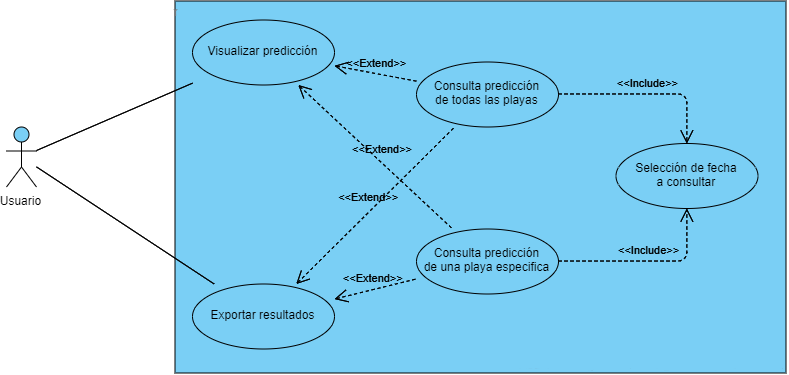
\includegraphics[width=1.1\textwidth]{DiagramaCasosUso.png}
	\caption{Diagrama de casos de uso}\label{fig:casos}
\end{figure}

	\subsection{Casos de uso}

\tablaSmallSinColores{Caso de uso 1: Visualizar predicción}{p{3cm} p{.75cm} p{9cm}}{tablaCUX}{
	\multicolumn{3}{p{10.25cm}}{CU-1: Visualizar predicción} \\
}
{
	Descripción                            & \multicolumn{2}{p{10.25cm}}{Permite al usuario visualizar toda la información relativa a la consulta realizada.} \\\cline{1-3}
	\multirow{0}{3.5cm}{Pre-condiciones} &\multicolumn{2}{p{10.25cm}}{La fecha introducida, es una fecha válida.} \\\cline{2-3}
	&\multicolumn{2}{p{10.25cm}}{El nombre de la playa introducida, es un nombre válido.} \\\cline{1-3}
	Requisitos                         	   & \multicolumn{2}{p{10.25cm}}{RF-5, RF-6} \\\cline{1-3}
	\multirow{0}{3.5cm}{Secuencia normal}  & Paso & Acción \\\cline{2-3}
	& 1    & El usuario debe acceder a la pestaña <<Mapas>>. \\\cline{2-3}
	& 2    & El usuario introduce una fecha.  \\\cline{2-3}
	& 3	   & El usuario podría elegir una playa en particular si lo desea o hacer una búsqueda general. \\\cline{2-3}
	& 4	   & El usuario pulsa el botón de búsqueda. \\\cline{2-3}
	& 5	   & Se muestra por pantalla el resultado de la consulta. \\\cline{1-3}
	Excepciones & 1 & Fecha introducida no válida. \\\cline{1-3}
	Frecuencia                             & Alta \\\cline{1-3}
	Importancia                            & Alta \\
}
	
\tablaSmallSinColores{Caso de uso 2: Exportar resultados}{p{3cm} p{.75cm} p{9cm}}{tablaCUX}{
	\multicolumn{3}{p{10.25cm}}{CU-2: Exportar resultados} \\
}
{
	Descripción                            & \multicolumn{2}{p{10.25cm}}{Permite al usuario descargar el resultado de la consulta.} \\\cline{1-3}
	\multirow{0}{3.5cm}{Pre-condiciones} &\multicolumn{2}{p{10.25cm}}{La fecha introducida, es una fecha válida.} \\\cline{2-3}
    &\multicolumn{2}{p{10.25cm}}{El nombre de la playa introducida, es un nombre válido.} \\\cline{1-3}
	Requisitos                         	   & \multicolumn{2}{p{10.25cm}}{RF-6, RF-7} \\\cline{1-3}
	\multirow{3}{3.5cm}{Secuencia normal}  & Paso & Acción \\\cline{2-3}
	& 1    & El usuario debe acceder a la pestaña <<Mapas>>. \\\cline{2-3}
	& 2    & El usuario introduce una fecha.  \\\cline{2-3}
	& 3	   & El usuario podría elegir una playa en particular si lo desea o hacer una búsqueda general. \\\cline{2-3}
	& 4	   & El usuario pulsa el botón de búsqueda. \\\cline{2-3}
	& 5	   & Se muestra por pantalla el resultado de la consulta. \\\cline{2-3}
	& 6    & El usuario pulsa el botón de descarga.\\\cline{2-3}
	& 7    & El archivo se descarga en el dispositivo.\\\cline{1-3}
	Excepciones & 1 & Fecha introducida no válida. \\\cline{1-3}
	Frecuencia                             & Baja \\\cline{1-3}
	Importancia                            & Alta \\
}

\tablaSmallSinColores{Caso de uso 3: Visualización del mapa}{p{3cm} p{.75cm} p{9cm}}{tablaCUX}{
	\multicolumn{3}{p{10.25cm}}{CU-3: Visualización del mapa} \\
}
{
	Descripción                            & \multicolumn{2}{p{10.25cm}}{Permite al usuario visualizar un mapa sobre el que se superpondrán los datos} \\\cline{1-3}
	Pre-condiciones                         & \multicolumn{2}{p{10.25cm}}{-} \\\cline{1-3}
	Requisitos                         	   & \multicolumn{2}{p{10.25cm}}{RF-5} \\\cline{1-3}
	\multirow{3}{3.5cm}{Secuencia normal}  & Paso & Acción \\\cline{2-3}
	& 1    & El usuario debe acceder a la pestaña <<Mapas>>. \\\cline{2-3}
	& 2    & Se muestra la ventana de consultas en la que aparece el mapa. \\\cline{1-3}
	Excepciones							   & - \\\cline{1-3}
	Frecuencia                             & Alta \\\cline{1-3}
	Importancia                            & Alta \\
}

\tablaSmallSinColores{Caso de uso 4: Consulta predicción}{p{3cm} p{.75cm} p{9cm}}{tablaCUX}{
	\multicolumn{3}{p{10.25cm}}{CU-4: Consultar predicción} \\
}
{
	Descripción                            & \multicolumn{2}{p{10.25cm}}{Permite al usuario realizar una consulta.} \\\cline{1-3}
	\multirow{0}{3.5cm}{Pre-condiciones} &\multicolumn{2}{p{10.25cm}}{La fecha introducida, es una fecha válida.} \\\cline{2-3}
	&\multicolumn{2}{p{10.25cm}}{El nombre de la playa introducida, es un nombre válido.} \\\cline{1-3}
	Requisitos                         	   & \multicolumn{2}{p{10.25cm}}{RF-4} \\\cline{1-3}
	\multirow{0}{3.5cm}{Secuencia normal}  & Paso & Acción \\\cline{2-3}
	& 1    & El usuario debe acceder a la pestaña <<Mapas>>. \\\cline{2-3}
	& 2    & El usuario introduce una fecha.  \\\cline{2-3}
	& 3	   & El usuario podría elegir una playa en particular si lo desea o hacer una búsqueda general. \\\cline{2-3}
	& 4	   & El usuario pulsa el botón de búsqueda. \\\cline{1-3}
	\multirow{0}{3.5cm}{Excepciones} & 1 & Fecha introducida no válida. \\\cline{2-3}
	& 2 & Las coordenadas no existen o no son válidas.  \\\cline{1-3}
	Frecuencia                             & Alta \\\cline{1-3}
	Importancia                            & Alta \\
}

\tablaSmallSinColores{Caso de uso 4.1: Consulta modelo predictivo}{p{3cm} p{.75cm} p{9cm}}{tablaCUX}{
	\multicolumn{3}{p{10.25cm}}{CU-4.1: Consultar modelo predictivo} \\
}
{
	Descripción                            & \multicolumn{2}{p{10.25cm}}{La aplicación web realiza  una consulta al modelo predictivo con los parámetros marcados por el usuario.} \\\cline{1-3}
	Pre-condiciones &\multicolumn{2}{p{10.25cm}}{-} \\\cline{1-3}
	Requisitos                         	   & \multicolumn{2}{p{10.25cm}}{RF-4} \\\cline{1-3}
	\multirow{0}{3.5cm}{Secuencia normal}  & Paso & Acción \\\cline{2-3}
	& 1    & La aplicación web realiza una llamada al modelo predictivo. \\\cline{2-3}
	& 2    & El modelo devuelve el resultado de la consulta.  \\\cline{2-3}
	& 3	   & La aplicación web imprime por pantalla dichos resultados. \\\cline{1-3}
	\multirow{0}{3.5cm}{Excepciones} & 1 & Fecha introducida no válida. \\\cline{2-3}
	& 2 & Las coordenadas no existen o no son válidas.  \\\cline{1-3}
	Frecuencia                             & Alta \\\cline{1-3}
	Importancia                            & Alta \\
}

\tablaSmallSinColores{Caso de uso 4.2: Selección de la fecha a consultar}{p{3cm} p{.75cm} p{9cm}}{tablaCUX}{
	\multicolumn{3}{p{10.25cm}}{CU-4.2: Selección de la fecha la consultar} \\
}
{
	Descripción                            & \multicolumn{2}{p{10.25cm}}{El usuario elige una fecha en la que realizar a consulta.} \\\cline{1-3}
	Pre-condiciones &\multicolumn{2}{p{10.25cm}}{-} \\\cline{1-3}
	Requisitos                         	   & \multicolumn{2}{p{10.25cm}}{RF-4} \\\cline{1-3}
	\multirow{0}{3.5cm}{Secuencia normal}  & Paso & Acción \\\cline{2-3}
	& 1    & El usuario debe acceder a la pestaña <<Mapas>>. \\\cline{2-3}
	& 2    & El usuario introduce una fecha.  \\\cline{1-3}
	Excepciones & 1 & Fecha introducida no válida. \\\cline{1-3}
	Frecuencia                             & Alta \\\cline{1-3}
	Importancia                            & Alta \\
}